\documentclass[tikz,border=8pt]{standalone}

\usepackage[T1]{fontenc}
\usepackage{helvet}
\renewcommand{\familydefault}{\sfdefault}
\usetikzlibrary{arrows.meta,backgrounds,fit,positioning}

\definecolor{ink}{HTML}{253238}
\definecolor{line}{HTML}{526A72}
\definecolor{sourcefill}{HTML}{F4E7CF}
\definecolor{processfill}{HTML}{DDEFF2}
\definecolor{storefill}{HTML}{E0EAD2}
\definecolor{runtimefill}{HTML}{D9E8E6}
\definecolor{outputfill}{HTML}{F3DFA2}
\definecolor{supportfill}{HTML}{ECEFF1}
\definecolor{laneoffline}{HTML}{F7FAFA}
\definecolor{laneruntime}{HTML}{F6F8F3}

\begin{document}
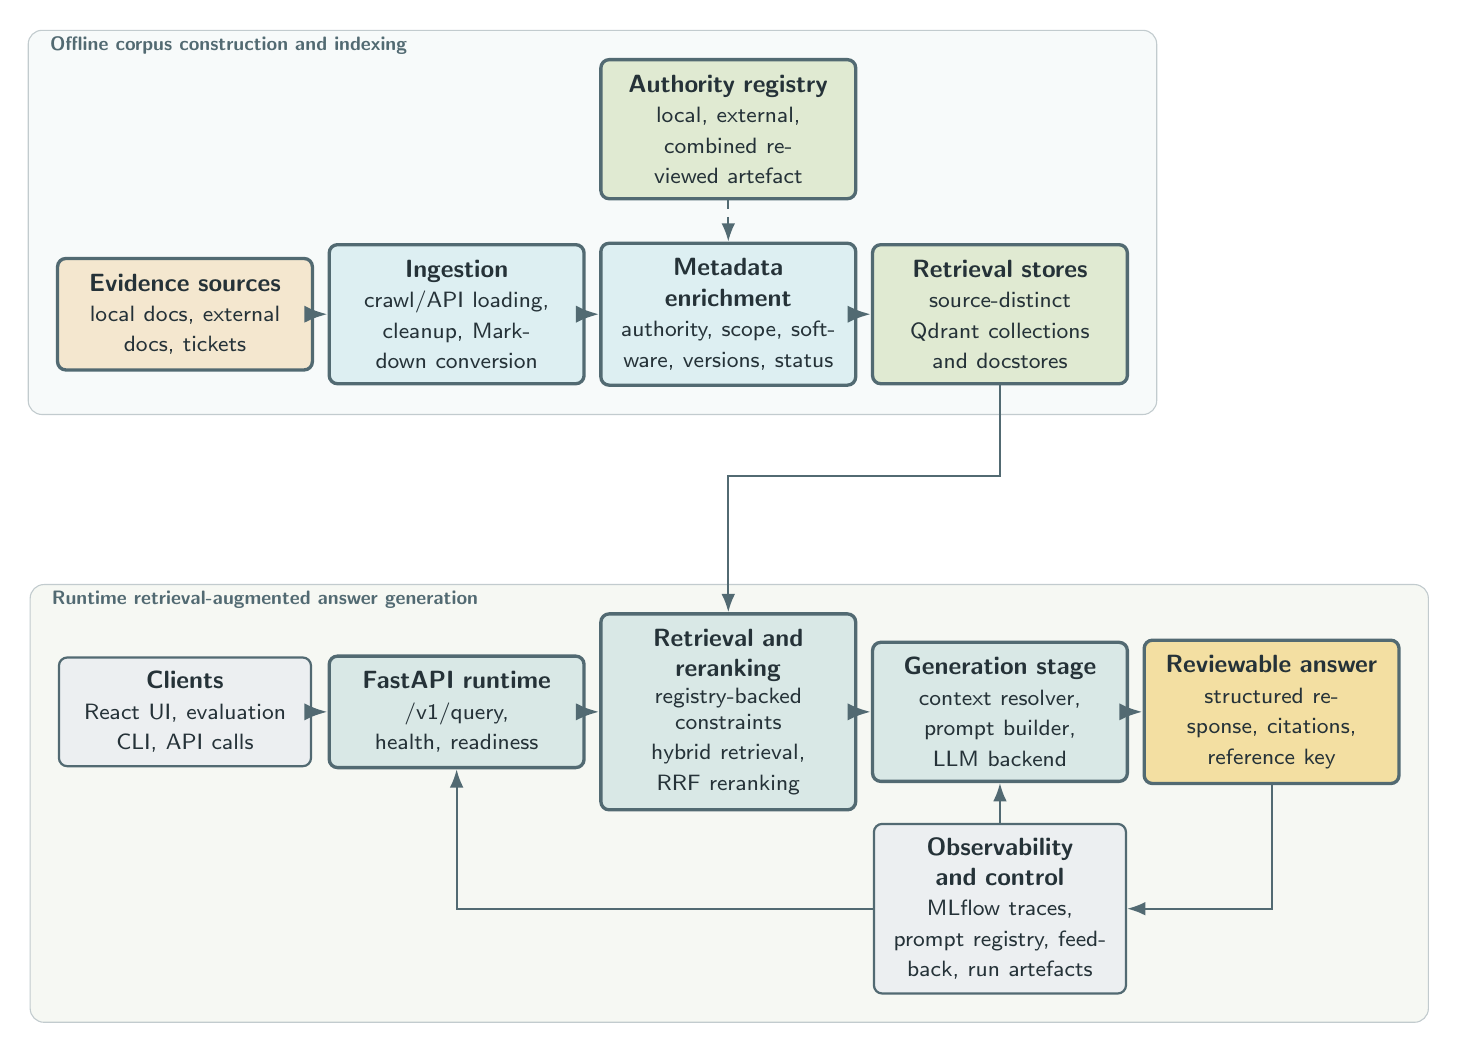
\begin{tikzpicture}[
  font=\small,
  text=ink,
  box/.style={
    draw=line,
    very thick,
    rounded corners=3pt,
    align=center,
    inner sep=5.5pt,
    minimum height=1.18cm,
    text width=2.85cm
  },
  compact/.style={
    draw=line,
    thick,
    rounded corners=3pt,
    align=center,
    inner sep=5pt,
    minimum height=1.00cm,
    text width=2.85cm
  },
  source/.style={box, fill=sourcefill},
  process/.style={box, fill=processfill},
  store/.style={box, fill=storefill},
  runtime/.style={box, fill=runtimefill},
  output/.style={box, fill=outputfill},
  support/.style={compact, fill=supportfill},
  arrow/.style={-Latex, very thick, draw=line},
  dataarrow/.style={-Latex, thick, draw=line},
  metaarrow/.style={-Latex, thick, dashed, draw=line},
  note/.style={font=\scriptsize, text=line, align=center},
  lane/.style={
    draw=line!35,
    rounded corners=5pt,
    fill=#1,
    inner sep=10pt
  }
]

% Offline construction path
\node[source] (sources) at (0,3.75) {\textbf{Evidence sources}\\{\footnotesize local docs, external docs, tickets}};
\node[process] (ingest) at (3.45,3.75) {\textbf{Ingestion}\\{\footnotesize crawl/API loading, cleanup, Markdown conversion}};
\node[process] (enrich) at (6.90,3.75) {\textbf{Metadata enrichment}\\{\footnotesize authority, scope, software, versions, status}};
\node[store] (stores) at (10.35,3.75) {\textbf{Retrieval stores}\\{\footnotesize source-distinct Qdrant collections and docstores}};
\node[store] (registry) at (6.90,6.10) {\textbf{Authority registry}\\{\footnotesize local, external, combined reviewed artefact}};

\draw[arrow] (sources) -- (ingest);
\draw[arrow] (ingest) -- (enrich);
\draw[arrow] (enrich) -- (stores);
\draw[metaarrow] (registry.south) -- (enrich.north);

% Runtime query path
\node[support] (clients) at (0,-1.30) {\textbf{Clients}\\{\footnotesize React UI, evaluation CLI, API calls}};
\node[runtime] (api) at (3.45,-1.30) {\textbf{FastAPI runtime}\\{\footnotesize /v1/query, health, readiness}};
\node[runtime] (retrieval) at (6.90,-1.30) {\textbf{Retrieval and reranking}\\{\footnotesize registry-backed constraints\\hybrid retrieval, RRF reranking}};
\node[runtime] (generation) at (10.35,-1.30) {\textbf{Generation stage}\\{\footnotesize context resolver, prompt builder, LLM backend}};
\node[output] (answer) at (13.80,-1.30) {\textbf{Reviewable answer}\\{\footnotesize structured response, citations, reference key}};
\node[support] (observability) at (10.35,-3.80) {\textbf{Observability and control}\\{\footnotesize MLflow traces, prompt registry, feedback, run artefacts}};

\draw[arrow] (clients) -- (api);
\draw[arrow] (api) -- (retrieval);
\draw[arrow] (retrieval) -- (generation);
\draw[arrow] (generation) -- (answer);

\draw[dataarrow] (stores.south) -- ++(0,-1.15) -| (retrieval.north);
\draw[dataarrow] (observability.west) -| (api.south);
\draw[dataarrow] (observability.north) -- (generation.south);
\draw[dataarrow] (answer.south) |- (observability.east);

% Lane backgrounds
\begin{scope}[on background layer]
  \node[lane=laneoffline, fit=(sources)(ingest)(enrich)(registry)(stores)] (offlinebox) {};
  \node[lane=laneruntime, fit=(clients)(api)(retrieval)(generation)(answer)(observability)] (runtimebox) {};
\end{scope}

\node[note, anchor=west] at ([xshift=0.16cm,yshift=-0.20cm]offlinebox.north west) {\textbf{Offline corpus construction and indexing}};
\node[note, anchor=west] at ([xshift=0.16cm,yshift=-0.20cm]runtimebox.north west) {\textbf{Runtime retrieval-augmented answer generation}};

\end{tikzpicture}
\end{document}
